%%%%%%%%%%%%%%%% based on Springer template for conference proceedings %%%%%%%%%%%%%%%%%%%%%%%%%%%%%%%%%%


\documentclass{svproc}


% to typeset URLs, URIs, and DOIs
\usepackage{url}
\usepackage[T1]{fontenc}
\usepackage[utf8]{inputenc}
\usepackage[english]{babel}
\usepackage{csquotes}

\usepackage{hyperref}
\usepackage{amssymb}
\usepackage{amsmath}
\usepackage{cleveref}
\usepackage{bm}
\usepackage{mathtools}
\usepackage{siunitx}
\usepackage{subfig}
\usepackage{graphicx}
\usepackage{epstopdf}
\usepackage{tabularx}
\usepackage{algorithm}
\usepackage{algpseudocode}
\usepackage{array}
\usepackage{booktabs}
\usepackage{multicol}
\usepackage{xcolor}
\usepackage[title]{appendix}
\usepackage{empheq}


\def\UrlFont{\rmfamily}

\newcommand{\vect}[1]{\bm{#1}}
\newcommand{\mat}[1]{#1}
\newcommand{\norm}[1]{\left\lVert#1\right\rVert}



%%%%%%%%%%%%%%%%%%%%%%%%%%%%%%%%%%%%%%%%%%%%%%%%%%%%%%%%%%5


\begin{document}
\mainmatter              % start of a contribution
%
\title{Solving Non-smooth Dynamic Problems using \\ the 
Alternating Direction Method of Multipliers}
%
\titlerunning{Non-smooth dynamic problem}  % abbreviated title (for running head)
%                                     also used for the TOC unless
%                                     \toctitle is used
%
\author{Alessandro Tasora \and Dario Mangoni \and Simone Benatti}
%
\authorrunning{Alessandro Tasora et al.} % abbreviated author list (for running head)
%
%%%% list of authors for the TOC (use if author list has to be modified)
\tocauthor{Alessandro Tasora, Dario Mangoni, and Simone Benatti}
%
\institute{University of Parma, Department of Engineering and Architecture \\ V.le delle Scienze 181/A, 40121 ITALY\\
\email{alessandro.tasora@unipr.it},\\ WWW home page:
\texttt{http://digitaldynamicslab.unipr.it}
}

\maketitle              % typeset the title of the contribution

\begin{abstract}
We propose to use the Alternating Direction Method of Multipliers (ADMM) for solving the variational inequality that arises in non-smooth contact problems in multibody simulations. The ADMM method is based on simple computational primitives and offers good convergence properties especially for scenarios where loose tolerance on the precision can be accepted, thus making it attractive also for real-time applications. The method scales well with the problem size and require a small number of tuning parameters. Differently from other methods known in literature, such as fixed point iterations, it can easily handle problems that mix finite elements and rigid bodies, and it is only marginally affected by odd mass ratios or ill-posed problems. Another attractive feature is that it can be easily warm-started.
\keywords{ADMM, non-smooth dynamics, contact}
\end{abstract}
%




%%%%%%%%%%%%%%%%%%%%%%%%%%%%%%%%%%%%%%%%%%%%%%%%%%%%%%%%%%%%


\section{Introduction}

Following the seminal works by Moreau 
\cite{mor88,Jean1992} 
most formulations for non-smooth dynamical problems are based on Measure Differential Inclusions: just like differential inclusions they allow set-valued force laws (such as the Coulomb-Amontons dry friction model) but also generalize to the case where velocity is assumed to be a possibly discontinuous function of bounded variation in order to allow impulsive events.

These problems can be solved by means of special time stepping methods that offer superior robustness and stability at the cost of solving a complementarity problem, or more in general a Variational Inequality (VI), per each time step
 \cite{acary2008numerical}. 
In this context, unknowns to be solved are velocity measures and reaction impulses at contact points and at joints: in cases of many parts with lot of frictional contacts, the large dimension of the VI could lead to a bottleneck in the time stepping process. This stimulated lot of research on efficient numerical methods in the last three decades.  

One of the former approaches, presented in 
\cite{StTr95}  % LCP solved via Lemke
, was based on solving a Linear Complementarity Problem (LCP) per each time step. LCPs are sub cases of VIs, for whom a direct method (Lemke algorithm) does exist. However, direct LCP solvers offer exact solution at the cost of very expensive pivoting sub iterations that scale badly with increasing number of unknowns, and for these reason they are not much used nowadays.

On the other hand, approximate but efficient methods based on fixed-point iterations became popular in the area of real-time simulators and robotics \cite{Bender2014}.
In most cases they are based on stationary methods like Gauss-Seidell or Jacobi iterations interleaved with projections on friction cones. They can be used to solve the LCP or the Cone Complementarity Problem (CCP), another special case of the VI in which the multibody contact problem can be formulated.
Attempts were made in order to parallelize them and to increase their convergence, such as over-relaxation, Krasnoselskii-Mann smoothing and warm starting, 
\cite{massSplittingRichard2012,TasoraAnitescuCMAME10} % P-GS iteration
but in general they perform poorly when there are odd mass ratios, and when articulated mechanisms such as robots are added to the scenarios - in those cases convergence often stalls, and if the iteration is prematurely truncated, reaction impulses are badly estimated and mechanisms fall apart or bend, and objects might interpenetrate. 

Another option is to solve the CCP as an optimization problem, using first-order optimization methods such as 
the Nesterov accelerated projected gradient descend  
\cite{hammadTOG2015}
or the Barzilai-Borwein spectral projected gradient
\cite{heynIJNME2013}. These methods are based on a simple projection operator,  matrix-by-vector multiplications and inner products. Their convergence is better than for fixed points iterations, however they share with them the following issue: that they often require the building of a Delassus operator, a matrix that is easy to compute in efficient (factored and sparse) format if diagonal masses are used because these can be easily inverted, but hard to handle if finite elements are added to the problem, because they introduce stiffness and damping matrices whose inverse would be needed as well.

A further class of solvers is represented by non-smooth newton methods, such as the one presented in 
\cite{Macklin2019} % Non-smooth Newton Method
, that assume a generic Nonlinear Complemetarity Problem (NCP), again a sub case of a VI, and represent the NCP complementarity constraints using non-smooth functions like the Fisher-Burmeister function. A generalized non-smooth Newton method can be used to find the zero of the functions, at the cost of solving a linear system per each iteration.

Under mild assumptions, the VI can be stated as a convex CCP, that can be also cast as an optimization problem, namely a Quadratic Program (QP) with convex constraints \cite{anitescuTasora2008}. For such a class of optimization problems, one can use Interior Point Methods (IPMs), a class of solvers that share some similarities with the above mentioned non-smooth Newton methods - for example the solution of a saddle-point linear system is required at each iteration. IPMs offer the best theoretical convergence. However, their implementation is quite intricate, and despite the encouraging theoretical properties, in practice they do not scale well for large problems. Also, there are no reliable ways to warm-start them
\cite{Mangoni2018}
.

Recently there has been a revival of Alternating Direction Method of Multipliers (ADMM) and similar operator-splitting methods for solving constrained optimization problems
\cite{Goldstein2014}. %  [2014 Alternating Direction Optimization Methods]. 
Even if the theoretical convergence of such methods is worse than the one of IPMs, recent developments showed that in practical scenarios they offer superior speed, scalability and robustness 
\cite{Cannon2019}. % [COSMO  conic operator splitting method for large convex problems].
An attractive property of ADMM is that it requires the solution of a linear system per each iteration, but unlike IPMs, such linear system most often remains unchanged during the iterations, so a factorization can be reused multiple times with a great benefit in terms of speed.

In 
\cite{Stellato2020} % [OSQP: an operator splitting solver for quadratic programs].
a specialized ADMM method for quadratic problems with conic constraints has been presented: on the top of this method we develop a solver that can exploit the nature of non-smooth dynamical problems. In our embodiment, unknowns are primal variables (velocity measures) and dual variables (impulses in contact points and joints), cone constraints stem from the Coulomb friction law, and the system matrix includes terms from the mass matrices and from the tangent stiffness/damping matrices (hence it is sparse, but not necessarily diagonal).

This paper will present a model for the non-smooth dynamics, it will show how to cast it as a QP with convex conic constraint, it will present the ADMM method to solve it, it will discuss practical implementation details and then it will show some benchmarks.

%%%%%%%%%%%%%%%%%%%%%%%%%%%%%%%%%%%%%%%%%%%%%%%%%%%%%%%5


\section{The non-smooth multibody model}

From \cite{TasoraAnitescuCMAME10} one can see that the non-smooth DVI after regularization and convexification turns into this: at each time step one has to solve the following (mixed) Cone Complementarity Problem:

\begin{subequations}
	\begin{empheq}[left=\empheqlbrace]{align}
    M \vect{v} - \vect{k} - D_\epsilon \bar{\vect{\gamma}}_\epsilon &= 0 \\
    D_{\epsilon}^T \vect{v}  + \vect{b}_\epsilon &= \vect{u}_\epsilon\\
    -\Upsilon^{\circ} \ni \vect{u}_\epsilon  \quad \bot &\quad  \bar{\vect{\gamma}}_\epsilon \in \Upsilon
	\end{empheq}
	\label{eq:ChronoMCCP}
\end{subequations}

where 
\begin{itemize}
    \item $M$ is a positive definite, block diagonal matrix containing masses and inertia tensors of the bodies
    \item $D_\epsilon$ is a sparse matrix, the transpose jacobian of all constraints
    \item $\vect{k}$ is a vector containing terms proportional to applied forces, among other things 
    \item $\vect{b}$ is a vector containing constraint stabilization terms, among other things
    \item $\Upsilon$ is the Cartesian product of all cones of admissible constraint forces, $\Upsilon = \bigtimes_i \Upsilon_i$
    \item if a frictional contact is added, $\Upsilon_i \subset \mathbb{R}^3$ is a second order Lorentz cone with aperture proportional to friction coefficient
    \item if a bilateral constraint is added, $\Upsilon_i = \mathbb{R}$ and $\Upsilon^\circ_i = \{0\}$
    \item if a unilateral constraint is added, $\Upsilon_i = \mathbb{R}^+$ and $\Upsilon^\circ_i = \mathbb{R}^-$
    \item $\Upsilon^{\circ}$ is the polar cone, opposite of the dual cone, i.e. $\Upsilon^{*} = -\Upsilon^\circ$.
\end{itemize}


For more details on the model we refer to 
\cite{negrutSerbanTasoraJCND2017}. % Posing Multibody Dynamics with Friction and Contact as a Differential Complementarity Problem

...


[TO REWRITE THE FOLLOWING]

By introducing the Schur complement 
\[
N=D_{\epsilon}^T M^{-1} D_{\epsilon}
\]
and the vector
\[
\vect{r}_\epsilon = D_{\epsilon}^T M^{-1} \vect{k} + \vect{b}_\epsilon
\]
such that
\[
\vect{u}_\epsilon = N \bar{\vect{\gamma}}_\epsilon + \vect{r}_\epsilon \, , 
\]
one can also write the problem as the following CCP:
\begin{align}
    -\Upsilon^{\circ} \ni  N \bar{\vect{\gamma}}_\epsilon + \vect{r}_\epsilon 
    \quad \bot \quad  
    \bar{\vect{\gamma}}_\epsilon \in \Upsilon
	\label{eq:ChronoCCP}
\end{align}

This CCP corresponds, again, to a first order optimality condition of a convex quadratic program, but this time of the type
\begin{subequations}
	\begin{empheq}[box=\fbox]{align}
	\text{min} \quad & \frac{1}{2} \bar{\vect{\gamma}}_\epsilon^T N \bar{\vect{\gamma}}_\epsilon + \vect{r}^T_\epsilon \bar{\vect{\gamma}}_\epsilon \\
	\text{s.t.} \quad & \bar{\vect{\gamma}}_\epsilon \in \Upsilon
	\end{empheq}
	\label{eq:ChronoCCP_min}
\end{subequations}
%
and in fact, the CCP \eqref{eq:ChronoCCP} can be written in the more conventional language of the KKT optimality conditions introducing $\vect{y}$ multipliers, for $\vect{y}=-\vect{u}_\epsilon$:
\begin{subequations}
	\begin{align}
    N \bar{\vect{\gamma}}_\epsilon + \vect{r}_\epsilon + I \vect{y} &= 0 \\
    \bar{\vect{\gamma}}_\epsilon &= \vect{z} \\
    \Upsilon \ni \vect{z}  \quad \bot &\quad \vect{y} \in \Upsilon^\circ % \mathcal{N}(\Upsilon)
	\end{align}
	\label{eq:ChronoCCP_kkt}
\end{subequations}

Also in this case, efficient methods like ADMM can be used to solve the convex program \eqref{eq:ChronoCCP_min}. Differently from \eqref{eq:ChronoMCCP_min} in this case we would iterate to solve for unknown $\bar{\vect{\gamma}}_\epsilon$, and then compute $\vect{v} = M^{-1}( \vect{k} + \bar{D}_\epsilon \bar{\vect{\gamma}}_\epsilon)$ with a quick postprocessing step. We call this approach \textbf{IDEA "A"}.

In this approach, the ADMM method requires a fast way to perform a projection 
$\Pi_{\Upsilon}$ onto the friction cones $\Upsilon$.


\subsection{Generalization: multi-flexible problems and non-conic force functions}

In order to generalize the problem \eqref{eq:ChronoMCCP} we relax the assumption of $M$ being diagonal, and instead of $M$ we introduce a symmetric positive definite matrix $H$, not necessarily sparse, that contains linear combinations of stiffness and damping matrices, added to the mass matrix. Stiffness and damping matrices are needed when dealing with implicit integration of stiff forces as in FEA and compliant parts, in general they are block-sparse, anyway less sparse than the original $M$ matrix, thus rendering the computation of $H^{-1}$ much less friendly than computing $M^{-1}$.

As a second generalization, we assume that $\bar{\vect{\gamma}}_\epsilon$ is not constrained in a friction cone $\Upsilon$, but rather in a generic convex set $\mathcal{C}$. That is, we assume $\bar{\vect{\gamma}}_\epsilon \in \mathcal{C}$ and at the same time we assume an associated \footnote{Not all dissipative constitutive models are associated, for example in some computational plasticity models the plastic flow might deviate respect to the normal to the yeld surface, and the Coulmb contact model itself is not associated -in fact the contact velocity $\vect{u}$ can range into a wider cone than the polar of the friction cone, but our DVI model compensates fur such effect. We will assume associated models heretofore, and we do not deal with non-associated models to avoid additional complexity for the moment.} flow $\vect{u}_\epsilon \in - \mathcal{N}_{C}(\bar{\vect{\gamma}}_\epsilon)$.

Using generic $\mathcal{C}$ allows, for an example, a friction cone capped with some upper limit (ex to simulate plastic contacts that cannot withstand excessive pressure) or a friction cone shifted a bit downward (ex to simulate cohesion in contacts) etc.

Under this more general setting, the time stepping of the multibody model becomes:

\begin{subequations}
	\begin{empheq}[left=\empheqlbrace]{align}
    H \vect{v} - \vect{k} - {D}_\epsilon \bar{\vect{\gamma}}_\epsilon &= 0 \label{eq:ChronoVI_primal}\\
    {D}_{\epsilon}^T \vect{v}  + \vect{b}_\epsilon &= \vect{u}_\epsilon\\
    \bar{\vect{\gamma}}_\epsilon \in \mathcal{C} : \quad  \vect{u}_\epsilon &\in - \mathcal{N}_{C}(\bar{\vect{\gamma}}_\epsilon)  
	\end{empheq}
	\label{eq:ChronoVI}
\end{subequations}

This is a Variational Inequality (VI), and it contains the CCP of \eqref{eq:ChronoCCP_kkt} as a special case. In fact one can introduce a Schur matrix 
\[
N=D_{\epsilon}^T H^{-1} D_{\epsilon}
\] similarly to what presented in  IDEA "A", and rewrite it as:
\begin{subequations}
	\begin{align}
    N \bar{\vect{\gamma}}_\epsilon + \vect{r}_\epsilon - \vect{u}_\epsilon &= 0 \\
    \bar{\vect{\gamma}}_\epsilon \in \mathcal{C} : \quad  -\vect{u}_\epsilon &\in \mathcal{N}_{C}(\bar{\vect{\gamma}}_\epsilon) 
	\end{align}
	\label{eq:ChronoVI_schur}
\end{subequations}
Also, using the same symbols introduced in OSQP, with $\vect{y}=-\vect{u}_\epsilon$, one gets
\begin{subequations}
	\begin{align}
    N \bar{\vect{\gamma}}_\epsilon + \vect{r}_\epsilon + I \vect{y} &= 0 \\
    \bar{\vect{\gamma}}_\epsilon &= \vect{z} \\
    \vect{z} \in \mathcal{C} : \quad  \vect{y} &\in \mathcal{N}_{C}(\bar{\vect{\gamma}}_\epsilon) 
	\end{align}
	\label{eq:ChronoVI_schur_kkt}
\end{subequations}
where one can easily see that this is a VI$(\vect{y}(\bar{\vect{\gamma}}_\epsilon), \mathcal{C})$ and that this is also the first order optimality condition of a convex quadratic program:
\begin{subequations}
	\begin{empheq}[box=\fbox]{align}
	\text{min} \quad & \frac{1}{2} \bar{\vect{\gamma}}_\epsilon^T N \bar{\vect{\gamma}}_\epsilon + \vect{r}^T_\epsilon \bar{\vect{\gamma}}_\epsilon \\
	\text{s.t.} \quad & \bar{\vect{\gamma}}_\epsilon \in \mathcal{C}
	\end{empheq}
	\label{eq:ChronoVI2_min}
\end{subequations}

Again, it is possible to apply ADMM algorithms to solve the problem.





\section{The ADMM solver}

...

[TO REWRITE THE FOLLOWING]


The ADMM starts by stating a penalized objective function, that includes all the constraints by means of indicator functions:
\begin{subequations}
	\begin{align}
	\text{min} \quad & \frac{1}{2} \vect{v}^T M \vect{v} - \vect{k}^T\vect{v} + \mathcal{I}_{\bar{D}_{\epsilon}^T \vect{v} + \vect{b}_\epsilon  = \vect{u}_\epsilon} (\tilde{\vect{v}}, \tilde{\vect{u}}_\epsilon) +
	\mathcal{I}_{\mathcal{K}}(\vect{u}_\epsilon)\\
	\text{s.t.} \quad & (\tilde{\vect{v}}, \tilde{\vect{u}}_\epsilon) = (\vect{v}, \vect{u}_\epsilon)
	\end{align}
\end{subequations}
where $\mathcal{I}_{\bar{D}_{\epsilon}^T \vect{v} + \vect{b}_\epsilon  = \vect{u}_\epsilon}$ and $\mathcal{I}_{\mathcal{K}}$ are infinite if the constraint is violated and zero if not. This introduces a really strong barrier, yet non-smooth.

The associated augmented lagragian is then used to build a equality constrained QP problem that is in the form:
\begin{subequations}
	\begin{align}
	\text{min} \quad & \frac{1}{2} \tilde{\vect{v}}^T M \tilde{\vect{v}} - \vect{k}^T\tilde{\vect{v}} + \frac{\sigma}{2}\norm{\tilde{\vect{v}}-\vect{v}^k}^2 + \frac{\rho}{2}\norm{\tilde{\vect{u}_\epsilon}-\vect{u}_\epsilon^k + \frac{\bar{\vect{\gamma}}_\epsilon}{\rho}}^2\\
	\text{s.t.} \quad & \bar{D}_{\epsilon}^T \tilde{\vect{v}} + \vect{b}_\epsilon  = \vect{u}_\epsilon
	\end{align}
\end{subequations}
whose KKT conditions can be found as:
\begin{equation}
    \begin{bmatrix}
        M + \sigma I_n & \bar{D}_{\epsilon} \\
        \bar{D}_{\epsilon}^T & -\rho^{-1} I_m
    \end{bmatrix}
    \begin{bmatrix}
        \tilde{\vect{v}}^{k+1} \\
        \vect{\nu}^{k+1}
    \end{bmatrix}
    =
    \begin{bmatrix}
        \vect{k} + \sigma \vect{v}^k \\
        \vect{b}_\epsilon - \vect{u}_\epsilon^k + \rho^{-1}\bar{\vect{\gamma}}_\epsilon^k
    \end{bmatrix}
\end{equation}

then we can update variables as
\begin{subequations}
	\begin{align}
	\tilde{\vect{u}}_\epsilon^{k+1} &= \vect{u}_\epsilon^k - \rho^{-1}(\vect{\nu}^{k+1} + \bar{\vect{\gamma}}_\epsilon^k)\\
	\vect{v}^{k+1} &= \alpha \tilde{\vect{v}}^{k+1} + (1-\alpha) \vect{v}^k\\
	\vect{u}_\epsilon^{k+1} &= \Pi_\mathcal{K}( \alpha \tilde{\vect{u}_\epsilon}^{k+1} + (1-\alpha) \vect{u}_\epsilon^k + \rho^{-1} \bar{\vect{\gamma}}_\epsilon^k ) \\
	\bar{\vect{\gamma}}_\epsilon^{k+1} &= \bar{\vect{\gamma}}_\epsilon^k + \rho (  \alpha \tilde{\vect{u}_\epsilon}^{k+1} + (1-\alpha) \vect{u}_\epsilon^k - \vect{u}_\epsilon^{k+1} )
	\end{align}
\end{subequations}

...





\section{Results}

...

\begin{figure}[h!]
\centering
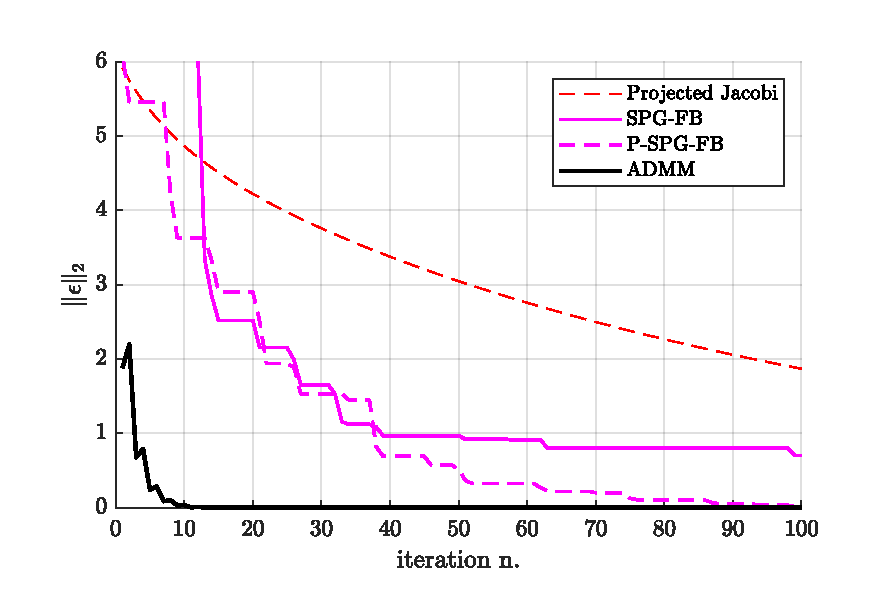
\includegraphics[width=0.50\textwidth]{t8_convergence.pdf}
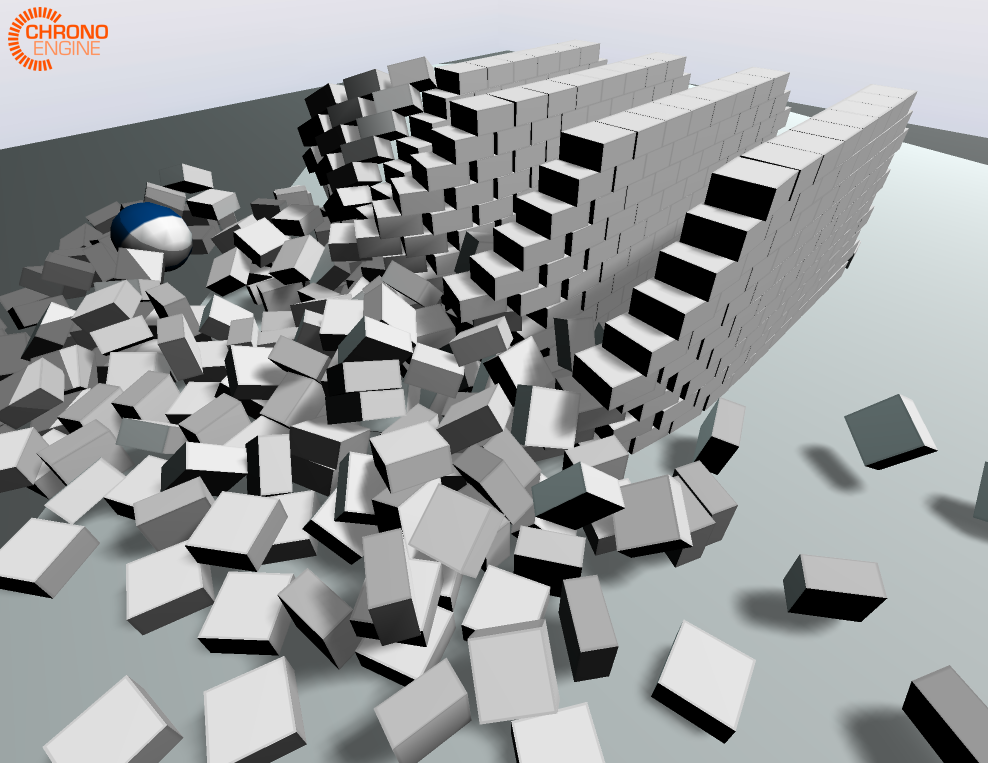
\includegraphics[width=0.35\textwidth, trim=0cm -3cm 0 3cm]{t8_snapshot.png}
\caption{Convergence of the ADMMM method within one time step of the wrecking ball benchmark (600 bricks in four walls): residual in frictional constraint   violation compared to fixed point Jacobi iterations and to first-order SPG methods.}
\end{figure}



\section{Conclusion}
 
Our ADMM method requires few computational primitives: basically a projection of dual variables on conic sets, a backward solve of a linear system, and a forward solve. The latter is a computational bottleneck, but it can be performed only once per run, as the matrix does not change often during the iterations. 
A good estimation of the ADMM step size proved to be fundamental in achieving good convergence: using some heuristics we obtained an efficient auto-tuning algorithm. 
We noted that ADMM can be successfully applied to problems that exhibit temporal coherence because, unlike IP methods, it supports warm-starting.





\bibliographystyle{spmpsci}
\bibliography{../../bibliography/refsMBS,../../bibliography/refsOPT}



\end{document}
